\documentclass[journal]{IEEEtran}
\usepackage{cite}
\usepackage{amsmath,amssymb}
\usepackage{graphicx}
\usepackage{url}
\def\UrlBreaks{\do\/\do-\do_}
\usepackage{array}
\usepackage{booktabs}
\usepackage{tikz}
\usetikzlibrary{positioning,arrows.meta,shapes.misc}
\usepackage[hidelinks]{hyperref}

\begin{document}
\bstctlcite{IEEEexample:BSTcontrol}

\title{Flood-Aware Urban Navigation Under Uncertain Evidence:\\ A Review of Routing, Road-Flood Sensing, Belief,\\ and Checked Explanation, with a Chennai Case}

\author{Pragatish~N,
        \textless Co-author~2\textgreater,
        and~\textless Co-author~3\textgreater%
\thanks{P.~N, \textless Co-author 2\textgreater{} and \textless Co-author 3\textgreater{} are with \textless Department\textgreater, Vellore Institute of Technology, Chennai, India (e-mail: \textless E-mail\textgreater).}%
\thanks{Second working draft, October 2026. Reference metadata were verified against Crossref, arXiv or publisher records; the verification log accompanies the draft.}}

\markboth{Working draft, October 2026}{N \MakeLowercase{\textit{et al.}}: Flood-Aware Urban Navigation Under Uncertain Evidence}

\maketitle

\begin{abstract}
Floods cut city road networks within hours, and the reports that could steer drivers around them are sparse, late, unevenly distributed and of mixed reliability. This review asks what research is available for a navigation system that routes on such evidence, states how sure it is, explains its choices without inventing facts, and keeps working when connectivity fails. We reviewed 323 works published between 1927 and 2026, each checked against a primary metadata record, and organised them into nine strands: flood impacts on road networks; flood-aware routing and evacuation; sensing of road flooding from crowds, images, vehicles and sensors; routing under uncertainty, risk and ambiguity; belief fusion, trust decay and calibration; explanation of routes and checking of generated text; language models for transport and disasters, including on-device models; offline-first systems and human reliance; and the Chennai and Indian context. Four findings stand out. First, almost every component has precedent, including flood-aware routing, decay of report trust, risk-averse path objectives and correctness of landmark search under rising weights. Second, flood routers usually take the flood state from a model as known; only a few fuse live sources, and we found none that lets the amount of evidence change the edge cost. Third, the most promising new evidence for street passability comes from vehicle traces and low-cost sensors, not from crowd reports, whose coverage tracks traffic volume and neighbourhood. Fourth, evaluation is the weakest link: road-flood predictors report discrimination but rarely calibration, and routers are scored against the same model that produced their costs. A replay study on the Chennai road network, summarised here, illustrates the last point: crowd reports added nothing measurable over a static susceptibility prior. We close with ten open problems.
\end{abstract}

\begin{IEEEkeywords}
Calibration, crowdsourcing, explainable artificial intelligence, flood hazards, mobile computing, route planning, uncertainty.
\end{IEEEkeywords}

\section{Introduction}
\IEEEPARstart{F}{looding} is one of the most common ways in which cities lose their road networks. Hydrodynamic studies of Shanghai~\cite{yin2016shanghai} and York~\cite{coles2017york}, and a city-scale study of emergency responders~\cite{green2017emergency}, show that moderate pluvial events disconnect parts of a city and lengthen emergency response. Analyses of the San Francisco Bay Area~\cite{kasmalkar2020floods} and Boston~\cite{suarez2005boston}, and of accessibility under extreme floods~\cite{papilloud2021vulnerability}, trace how local inundation becomes system-wide delay; a study in southern China reports that more than 40\% of road connectivity in its area is lost under a 1-in-100-year rainfall~\cite{zhou2022connectivity}. Network science adds that small local floods can trigger abrupt, large-scale failure~\cite{wang2019percolation}. Speed falls well before a road becomes impassable, which the depth--disruption function of Pregnolato \emph{et al.}~\cite{pregnolato2017depth} quantifies; preparedness studies build on it~\cite{arrighi2019preparedness}.

Chennai, India, shows the problem clearly. The December 2015 event has been studied for its rainfall~\cite{vanoldenborgh2016chennai,panda2022observed,dutta2024uncovering}, geospatial and anthropogenic drivers~\cite{seenirajan2017chennai,ramasamy2018geoanthropogenic}, land-use change~\cite{devi2019sprawl,rath2018study}, and forecastability~\cite{paul2026aerosols}; a comparison of the 2015 and 2023 floods combines radar imagery with reservoir releases~\cite{radhakrishnan2024chennai}, and a national inventory places such events in a longer record~\cite{saharia2021inventory}. These studies describe events. They do not provide the live, street-level information that a driver or an ambulance needs while water is rising.

Mainstream navigation has begun to fill part of the gap. Google reported that India produced more flood-related alerts on Google Maps in 2025 than any other country~\cite{ramani2025maps}, and Mappls lists waterlogging and flood alerts among its user report categories~\cite{mappls2026post}. In Chennai, a crowd flood map ran as a pilot from 2017 to 2019~\cite{urbanrisklab2019riskmap}. What remains unclear from the published record is how report-based evidence should change a route, how its reliability should be judged, and how a system should behave when reports are absent or stale.

A navigation system for these conditions needs four capabilities at once. It must \emph{route} on a road graph whose costs depend on uncertain hazard evidence. It must keep a \emph{belief} about each road that fuses a static susceptibility prior with timestamped reports of varying reliability, and whose probabilities are calibrated. It must \emph{explain} a detour without inventing facts. And it must do this \emph{offline}, because floods damage the communication networks on which cloud services rely.

Existing surveys cover one capability each: route planning~\cite{bast2016route}, evacuation~\cite{bayram2016evac,li2025overview}, robust and distributionally robust shortest paths~\cite{filippi2025survey}, social media in emergencies~\cite{imran2015social}, volunteered geographic information (VGI)~\cite{senaratne2017vgi}, crowdsourcing for urban flood monitoring~\cite{helmrich2021opportunities}, truth discovery~\cite{li2016truthsurvey}, hallucination~\cite{ji2023hallucination}, data-to-text generation~\cite{osuji2024d2t}, explainable artificial intelligence (XAI)~\cite{adadi2018xai,guidotti2018survey,gilpin2018explaining}, large language models (LLMs) in transport~\cite{wandelt2024its,nie2025llm4tr,yan2025llmtransport,zhang2024mobilityllm} and disasters~\cite{lei2025disaster,xu2025disasterreview,zhu2025urbandisaster}, and on-device models~\cite{xu2024ondevice,lu2024slmsurvey}. This review reads across them. Its contributions are:
\begin{itemize}
\item a taxonomy of nine strands relevant to offline, uncertainty-aware, explainable flood navigation, with what each offers and leaves open (Sections~\ref{sec:impacts}--\ref{sec:india});
\item a cross-strand comparison (Table~\ref{tab:strands}) that separates capabilities with strong precedent from open gaps;
\item an account of which commonly claimed novelties have prior art, and of what a replay study on Chennai data showed about one such design (Section~\ref{sec:synthesis});
\item ten open problems grounded in the Chennai setting (Section~\ref{sec:open}).
\end{itemize}

\section{Review Method}\label{sec:method}
The first version of this review drew 129 works from seven internal project reports and targeted searches. For this version we ran five further searches, one per theme (flood routing; uncertain and risk-aware routing; road-flood sensing; route explanation and LLMs; Chennai and India), through Crossref, Consensus and Exa, using combinations of the terms \emph{flood}, \emph{road network}, \emph{routing}, \emph{evacuation}, \emph{ambulance}, \emph{robust}, \emph{CVaR}, \emph{Canadian traveller}, \emph{exposure}, \emph{Waze}, \emph{floating car}, \emph{probe}, \emph{CCTV}, \emph{flood depth}, \emph{sensor}, \emph{under-reporting}, \emph{explanation}, \emph{data-to-text}, \emph{hallucination}, \emph{small language model}, \emph{Chennai} and \emph{India}. A candidate was kept if it reported a method, measurement, dataset or system relevant to a strand and its metadata could be confirmed. Every kept item was checked against a primary record (Crossref by DOI or arXiv for almost all; a publisher, patent or project page for a few). Four candidates were excluded: two 2026 arXiv benchmarks with inconsistent identifiers, a preprint without a confirmed journal version, and a paper whose event attribution we could not reconcile. The corpus has 323 works from 1927 to 2026. Where we read only a title or abstract, we describe the work at that level. The corpus comes from targeted search rather than exhaustive screening, so this is a structured review, not a systematic review in the PRISMA sense.

\begin{figure}[t]
\centering
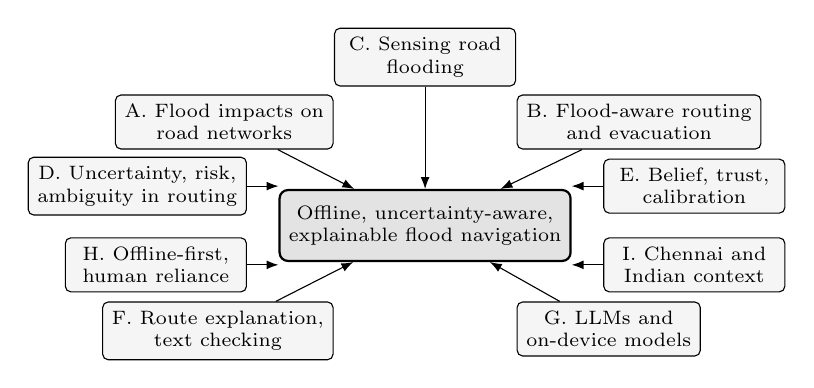
\begin{tikzpicture}[font=\scriptsize, node distance=2mm and 3mm,
  box/.style={draw, rounded corners=2pt, align=center, minimum width=2.3cm, minimum height=6mm, fill=gray!8},
  core/.style={draw, thick, rounded corners=3pt, align=center, minimum width=3.0cm, minimum height=9mm, fill=gray!22}]
\node[core] (c) {Offline, uncertainty-aware,\\explainable flood navigation};
\node[box, above left=5mm and -7mm of c] (a) {A. Flood impacts on\\road networks};
\node[box, above right=5mm and -7mm of c] (b) {B. Flood-aware routing\\and evacuation};
\node[box, above=13mm of c] (s) {C. Sensing road\\flooding};
\node[box, left=4mm of c, yshift=5mm] (cc) {D. Uncertainty, risk,\\ambiguity in routing};
\node[box, right=4mm of c, yshift=5mm] (d) {E. Belief, trust,\\calibration};
\node[box, left=4mm of c, yshift=-5mm] (g) {H. Offline-first,\\human reliance};
\node[box, right=4mm of c, yshift=-5mm] (h) {I. Chennai and\\Indian context};
\node[box, below left=5mm and -7mm of c] (e) {F. Route explanation,\\text checking};
\node[box, below right=5mm and -7mm of c] (f) {G. LLMs and\\on-device models};
\foreach \n in {a,b,s,e,f} \draw[-{Latex[length=1.5mm]}] (\n) -- (c);
\foreach \n in {cc,g} \draw[-{Latex[length=1.5mm]}] (\n.east) -- (c.west|-\n.east);
\foreach \n in {d,h} \draw[-{Latex[length=1.5mm]}] (\n.west) -- (c.east|-\n.west);
\end{tikzpicture}
\caption{Taxonomy used in this review. Each strand contributes one capability, or the setting, to the target system in the centre.}
\label{fig:taxonomy}
\end{figure}

\section{Background and Terminology}\label{sec:background}
A city is a directed graph $G=(V,E)$ with free-flow traversal time $\tau_0(e)$ on each edge. A \emph{hazard belief} $p(e,t)$ is the probability that edge $e$ is affected by a hazard class at time $t$. \emph{Evidence} consists of timestamped reports with a location, a polarity (present or cleared) and a source whose reliability may be known or estimated. A \emph{static prior} expresses susceptibility before any report; height above the nearest drainage (HAND)~\cite{nobre2011hand} and historical inundation maps are typical inputs. \emph{Calibration} means that, among edges assigned probability $q$, about a fraction $q$ are affected; it differs from \emph{discrimination}, which asks only whether affected edges score higher~\cite{fawcett2006roc}. An explanation is \emph{faithful} if it reflects the reasons the system used~\cite{jacovi2020faithful}; in a closed domain such as routing, a stricter and checkable requirement is that every factual token is grounded in the router's decision record. \emph{Risk} denotes known probabilities and \emph{ambiguity} uncertainty about the probabilities themselves~\cite{ellsberg1961risk}.

\section{Flood Impacts on Road Networks}\label{sec:impacts}
Coupled hydrodynamic and network models dominate this strand. Yin \emph{et al.}~\cite{yin2016shanghai} assess pluvial flash-flood risk to an intra-urban network; Coles \emph{et al.}~\cite{coles2017york} and Green \emph{et al.}~\cite{green2017emergency} model how far emergency responders can reach, moving the question from which streets flood to which people lose service. Zhou \emph{et al.}~\cite{zhou2022connectivity} couple one-dimensional drainage and two-dimensional inundation models. National-scale modelling for England shows that ambulance and fire services miss response-time targets more often even in modest floods~\cite{yu2020disruption}, and a Zhengzhou study attributes most deterioration of prehospital care to a mismatch between supply and demand~\cite{chen2025ems}. Compound surge and rainfall flooding has been quantified on roads with ambulance-positioning analysis under several depth thresholds~\cite{tahvildari2022compound}.

Network science explains why small floods matter. A failure model that reproduces most Hurricane Harvey road closures exhibits an abrupt phase transition in which local floods cause abrupt global failure~\cite{wang2019percolation}; percolation of Harvey traffic shows that a small fraction of failed segments shrinks the giant component sharply~\cite{dong2022modest}, and the effects of flooded segments persist for weeks and do not fade with distance~\cite{rajput2023anatomy}. An epidemic-style contagion model forecasts how road flooding spreads and recedes~\cite{fan2020contagion}, and a Bayesian network links channel overflow to road failure~\cite{dong2020bayesian}. Percolation and giant-component measures can mislead on high-resolution simulations, where accessibility partitions to critical services are more informative~\cite{loreti2022local}. Accessibility to amenities has been mapped for Iowa communities~\cite{alabbad2021iowa}, and topology-only vulnerability metrics have been proposed~\cite{morelli2021vulnerability}. Vehicle type matters: road functionality and emergency-vehicle access differ between cars and larger vehicles~\cite{he2024functionality,he2026ems}. Microscopic traffic simulation couples flood models with traffic models to estimate rerouted trips and lost hours~\cite{pyatkova2018micro}.

Two results matter for navigation. Disruption is gradual, so a router can slow an edge rather than delete it~\cite{pregnolato2017depth}; an Indian vulnerability study applied a depth--safe-speed curve and estimated that, in a 1-in-100-year event, over two-fifths of the road length could no longer be driven~\cite{singh2018vulnerability}. And the models are scenario tools, run for design storms with terrain and drainage data that many cities do not publish. Digital twins aim to make them interactive~\cite{kaynak2025twin,mandal2026flowsdt}, and global forecasting has improved from ensemble streamflow systems~\cite{alfieri2013glofas} to machine-learning prediction in ungauged basins~\cite{nearing2024global}, but these forecast rivers and catchments rather than streets.

\emph{What remains:} none of these works yields a street-level, time-stamped passability estimate that can be updated from reports during an event.

\section{Flood-Aware Routing and Evacuation}\label{sec:routing}
\subsection{Shortest paths and changing weights}
Dijkstra's algorithm~\cite{dijkstra1959note} and A* search~\cite{hart1968astar} remain the basis of most routers. Landmark search (ALT)~\cite{goldberg2005alt}, contraction hierarchies~\cite{geisberger2008ch} and customisable variants~\cite{dibbelt2016cch,delling2017crp} make large queries fast; Bast \emph{et al.}~\cite{bast2016route} survey the field, and time-dependent variants store shortcut paths rather than travel-time functions~\cite{strasser2021catchup}. OSRM brought these techniques to OpenStreetMap data~\cite{luxen2011osrm,haklay2008osm}. Hazard routing changes weights with every report. Customisable approaches separate metric-independent preprocessing from cheap customisation~\cite{dibbelt2016cch,delling2017crp}; Delling and Wagner showed that ALT ``still performs correct queries as long as an edge weight does not drop below its initial value''~\cite{delling2007landmark}, a property also used for bidirectional search on time-dependent networks~\cite{nannicini2012bidir}, and faster landmark preprocessing makes ALT usable under traffic updates~\cite{efentakis2013alt}. Incremental replanning after cost changes is the subject of D* Lite~\cite{koenig2005dstarlite}. Any hazard cost that never falls below free-flow time inherits ALT correctness from this literature.

\subsection{Routing on modelled floods}
Most flood routers take the flood state from a model. Studies plan risk-avoidance routes over a numerical flood model~\cite{li2023dijkstra}, combine routing with rescue dispatch~\cite{liang2025rescue}, learn rescue paths with reinforcement learning~\cite{li2025drl}, and route evacuation for dam-failure floods~\cite{an2025dam}. De~Faria \emph{et al.}~\cite{defaria2026routing} feed stormwater-model inundation for three hurricanes into a time-varying routing optimisation with flood--speed reductions. Panakkal \emph{et al.}~\cite{panakkal2023safer} couple live rainfall with a physical flood model and network analysis to report road conditions per vehicle class and loss of hospital access. Bucar and Hayeri learn a link flood-risk model from static terrain and drainage features and train a route assistant that balances length against reliability~\cite{bucar2022route}. Lupa \emph{et al.}~\cite{lupa2026stars} route ambulances on radar-derived passability; because radar and optical masks disagreed on impassable roads, they used both to bracket uncertainty. Web decision-support tools link river forecasts to precomputed inundation extents for routing and service areas~\cite{alabbad2024web}, and a graph neural surrogate speeds up shortest-distance estimation under probabilistic hurricane flooding~\cite{liu2025gnn}. On the industrial side, a flood-aware travel-routing application~\cite{ibm2013patent} and a patent on per-segment safety scores~\cite{uber2020patent} show the idea is not new.

\subsection{Evacuation}
Evacuation research adds capacity and timing~\cite{lu2005evac,bayram2016evac}, and a recent review covers simulation, shelters, route algorithms and evacuee behaviour~\cite{li2025overview}. Evacuation routes have been designed from neural-network flood prediction~\cite{lee2020evac}, cellular-automata optimisers with hydrodynamics~\cite{he2021cadro}, and pedestrian stability criteria~\cite{li2021pedestrian}. FLOAT trades travel time against flood exposure with tunable weights over simulated depths~\cite{jao2025float}. Multimodal water--ground emergency transport~\cite{song2025multimodal} and relief vehicle routing under flood likelihood~\cite{toathom2024vrp} extend the setting. Traffic simulation of Mumbai's Dadar area tests disruption and evacuation strategies~\cite{lalwani2025dadar}.

\subsection{Routing on observed or reported floods}
A smaller group routes on observations. Social-media events have been turned into a spatially decaying impedance field for hazard-aware routing~\cite{fu2026social}; crowd photos of stop signs give depths that are interpolated and avoided~\cite{alizadeh2021signs}; and a human--AI system combines gauge forecasts, HAND inundation and filtered social posts to select alternatives outside flooded areas~\cite{karanjit2026hac}. Panakkal and Padgett combine gauges, social media and imagery with physics models to infer link-level flood status~\cite{panakkal2024eyes}. An offline evacuation app treats a user's departure from the suggested path as a sign that a segment is blocked, reroutes, and shares the finding~\cite{itoi2017offline}; it is the closest prior work we found on traversal-derived evidence used offline.

\emph{What remains:} most flood routers assume a known, deterministic flood state. Those that use reports treat them as binary or spatially smoothed, and we found none that discounts reports by age and source and lets the amount of evidence change the cost.

\section{Sensing Road Flooding}\label{sec:sensing}
\subsection{Crowd reports and social media}
Goodchild's ``citizens as sensors''~\cite{goodchild2007citizens} and its disaster application~\cite{goodchild2010crowdsourcing} framed a large VGI literature; OpenStreetMap is its best-known product~\cite{haklay2008osm}, and quality-assessment methods have been reviewed~\cite{senaratne2017vgi}. Social media added a real-time channel: tweets detected earthquakes~\cite{sakaki2010earthquake}, emergency-message processing has been surveyed~\cite{imran2015social}, and combining posts with authoritative data improves the selection of useful messages~\cite{albuquerque2015geographic}. For floods, crowd and social observations have supported high-resolution urban monitoring~\cite{wang2018hyper}, rapid inundation mapping~\cite{rosser2017rapid,huang2018vgi,smith2017social}, flood modelling~\cite{assumpcao2018citizen}, and coastal severity modelling~\cite{sadler2018crowd}. Data assimilation of VGI into hydraulic models can persist~\cite{annis2019vgi}, whereas assimilated social data in another case gave only short-lived local gains~\cite{songchon2023assim}. Tweet quality can be scored~\cite{songchon2021quality}, and citizen-science projects report what made them work~\cite{lecoz2016citizen}. A review recommends integrating webcams, social media and citizen science~\cite{helmrich2021opportunities}.

\subsection{Navigation-app reports}
Waze reports have been assessed for reliability and coverage~\cite{aminnaseri2018waze}. Flood reports were checked for trustworthiness in Norfolk~\cite{praharaj2021waze}, used to estimate impacts of recurring flooding on vehicle travel~\cite{praharaj2021impacts}, matched to authoritative reports during Harvey by spatio-temporal clustering~\cite{lowrie2022waze}, and found in Dallas to align better with surface depressions than with hazard maps~\cite{safaei2023waze}. They serve as labels for road-flood prediction~\cite{yuan2023predicting,safaei2024hybrid,walker2024rfsi}, and crowd 3-1-1 reports can stand in for part of a physical sensor network~\cite{esparza2024crowd}. Three cautions follow. Video ground truth found sizeable false-alarm rates in Waze incident reports, with no correlation between Waze's reliability score and accuracy~\cite{goodall2019waze}. Coverage drifts with traffic volume~\cite{liu2023wazecoverage}. And reports under-represent some neighbourhoods~\cite{esparza2023imbalance,liu2024disparities}, which motivates models that correct for under-reporting~\cite{agostini2024underreport}.

\subsection{Vehicle traces}
Vehicles reveal flooding by what they do. Floating-car speeds combined with rainfall thresholds detect waterlogging~\cite{hu2018fcd}; loss of samples and speed anomalies detect flooded underpasses where change-point detection fails~\cite{song2015bridges}; drops in taxi passing rates~\cite{kong2022taxi} and GPS density~\cite{she2019gps} map flooded roads; probe-vehicle presence tracks inundation extent and speed falls with depth~\cite{hiramoto2025probe}; U-turn anomalies flag heavy-rain disruption~\cite{kawasaki2024uturn}; and a likelihood test on probe activity detects closures with high precision on low-volume roads~\cite{pietrobon2019closure}. Route selection for opportunistic sensing of waterlogging has also been studied~\cite{wang2024opportunity}, connected-vehicle wiper states estimate rainfall~\cite{bartos2019wipers}, and traffic-based nowcasting is part of community-scale flood monitoring~\cite{yuan2022smart}. Graph convolutional networks on speed data predict road flooding hours ahead~\cite{yuan2022stgcn}. These sources supply what crowd reports lack: evidence that a road is passable.

\subsection{Images and sensors}
Depth can be estimated from images of reference objects: stop signs~\cite{kharazi2021stopsign,alizadeh2023signage}, traffic signs~\cite{song2021floodmask}, submerged vehicle parts~\cite{zhong2024traffic}, and social-media photos with deep classifiers~\cite{wu2024cbam,du2025caresnet}, including a large multimodal model~\cite{akinboyewa2024gpt4v}; wheel contours in posted images have been proposed as a vehicle-as-gauge indicator~\cite{yang2026vfg}. Surveillance cameras give level trends~\cite{moydevitry2019sofi}, ponding levels~\cite{hao2022ponding}, flood extent~\cite{wang2024cctvseg} and river levels~\cite{vandaele2021river}, but image proxies with correlated errors can hurt model calibration~\cite{moydevitry2020proxy}. Low-cost street sensors measure depth directly: FloodNet deployed ultrasonic sensors across New York City~\cite{mydlarz2024floodnet}, stakeholders have described how they use such data~\cite{silverman2022waves}, and StormSense validated a street-level model with an IoT sensor network~\cite{loftis2018stormsense}. Physical and social sensing can be combined into an inundation probability map~\cite{du2024ips}.

\subsection{Combining sources}
Truth discovery estimates source reliability jointly with the truth, from the Dawid--Skene model~\cite{dawid1979em} to later methods~\cite{li2014crh,wang2012truth}, as surveyed in~\cite{li2016truthsurvey}.

\emph{What remains:} crowd reports cluster by event and neighbourhood and duplicate one another, yet fusion schemes often treat them as independent. Negative evidence, a road driven through without a report, is what a navigation app observes most often, and vehicle-trace studies show it can be measured, but we found no router that uses it as evidence of passability.

\section{Routing Under Uncertainty, Risk and Ambiguity}\label{sec:uncertain}
\subsection{Stochastic and reliable paths}
Early work defined shortest paths in probabilistic graphs~\cite{frank1969probabilistic}. Later studies addressed variance-constrained paths~\cite{sivakumar1994variance}, least-expected-time paths in dynamic networks~\cite{fu1998expected,millerhooks2000least}, path finding under uncertainty~\cite{chen2005pathfinding}, travel-time budgets with heterogeneous risk aversion~\cite{lo2006degradable}, on-time arrival~\cite{nie2009ontime}, most-reliable paths with correlated links~\cite{xing2011reliable}, risk-averse objectives~\cite{gavriel2012riskaverse}, and tractable reliable routing~\cite{samaranayake2012reliable}. Routing optimisation under uncertainty has been framed generally~\cite{jaillet2016routing}, and adaptive strategies that minimise the risk of exceeding a budget have robust versions for the case where only interval estimates of the cost statistics are available~\cite{flajolet2018robust}.

\subsection{Robust and distributionally robust paths}
Chance-constrained programming~\cite{charnes1959chance} and robust discrete optimisation~\cite{bertsimas2003robust} are the classical forms of caution. Robust shortest paths with interval data~\cite{yu1998robust,montemanni2004exact} were followed by distributionally robust models over moment-based~\cite{cheng2016drsp,zhang2018rsp,ketkov2021drsp} and Wasserstein ambiguity sets~\cite{wang2020wdrsp}; a recent survey classifies the field~\cite{filippi2025survey}.

\subsection{Risk measures and safety-aware navigation}
Hazardous-materials routing has long weighed cost against exposure~\cite{erkut1998hazmat}, including catastrophe-avoidance models~\cite{erkut2000catastrophe}, value-at-risk~\cite{kang2014var} and conditional value-at-risk on time-dependent networks~\cite{toumazis2013cvar}; worst-case CVaR addresses the case where historical data cannot pin down accident probabilities~\cite{toumazis2016wcvar}. Safety-aware navigation builds per-segment crime~\cite{galbrun2016safe} or crash risk~\cite{krumm2017riskaware,li2016roadrisk,ghoul2023safest} and trades it against time; an empirical-Bayes crash model with propagated exposure uncertainty reports large risk reductions at the cost of long detours~\cite{rohmann2026bayesian}. Exposure-aware routing is an instructive parallel. Air-pollution routing~\cite{sharker2014ape,mahajan2019car,zou2020healthier,wang2022activetravel,choudhary2022multimodal} and heat or shade routing~\cite{kolaxidis2025heat,wolf2025coolwalks,melnikov2022thermal} add an exposure term to travel time, much as a flood penalty does. Two results transfer: gains are largest where exposure varies sharply in space~\cite{zou2020healthier}, and on a regular grid with uniform building heights, a shade preference cannot beat the shortest path at all~\cite{wolf2025coolwalks}.

\subsection{Unknown blockages, learning and ambiguity}
When blocked roads are found only on arrival, the problem is the Canadian Traveller Problem~\cite{papadimitriou1991ctp}; stochastic shortest paths with recourse~\cite{polychronopoulos1996recourse} and uncertainty-aware policies~\cite{eyerich2010ctp} improve on optimistic replanning, and a risk-averse variant with correlated traversabilities produces information-seeking detours~\cite{lamarre2026riskctp}. Online routing learns travel times by bandit methods~\cite{talebi2018online,lagos2024online}, where upper confidence bounds encourage exploration~\cite{auer2002ucb}; offline reinforcement learning flips the bonus into a penalty and proves that such pessimism is efficient~\cite{jin2025pessimism}. Robotics uses CVaR constraints~\cite{hakobyan2019cvar} and learned risk-aware costmaps~\cite{fan2022costmaps}. Decision theory names the attitude: people prefer known risks to ambiguous ones~\cite{ellsberg1961risk}, and maxmin expected utility evaluates an action under the worst plausible prior~\cite{gilboa1989maxmin}.

\emph{What remains:} these formulations assume the uncertainty set or distribution is given. In flood routing it must be built from a handful of reports, and how its size should depend on evidence count, age and source is open.

\section{Belief, Trust Decay and Calibration}\label{sec:belief}
\subsection{Fusing evidence over time}
Occupancy grids established probabilistic fusion of noisy readings~\cite{elfes1989occupancy}, now usually implemented as additive log-odds updates. The persistence filter estimates whether a previously observed feature still exists~\cite{rosen2016persistence}, which is the question a navigation app faces for a reported flood. The beta reputation system with forgetting~\cite{josang2002beta}, subjective logic~\cite{josang2001logic} and trust surveys~\cite{josang2007survey} formalise reliability and its decay. Decay of trust with time is therefore well established.

\subsection{Pessimism and interval quality}
The normal-approximation (Wald) interval for a proportion behaves poorly near zero and one; the Wilson interval~\cite{wilson1927probable}, the Agresti--Coull interval~\cite{agresti1998approximate} and the comparison of Brown \emph{et al.}~\cite{brown2001interval} are better behaved. A pessimistic plug-in used by a router inherits these properties. In a Chennai replay, a Wald-type index with an evidence count in the denominator decreased after a single low-reliability report, because the band narrowed faster than the mean rose; a Bayesian upper quantile does not have this defect.

\subsection{Evaluating probabilities}
The Brier score~\cite{brier1950verification}, its decomposition~\cite{murphy1973partition}, forecaster comparison~\cite{degroot1983forecasters} and proper scoring rules~\cite{gneiting2007scoring} are standard. Machine learning revived calibration~\cite{niculescu2005predicting,naeini2015bbq,guo2017calibration} and documented pitfalls of expected calibration error~\cite{nixon2019calibration}. Receiver operating characteristic analysis measures discrimination separately~\cite{fawcett2006roc}. Road-flood predictors report discrimination, precision or recall~\cite{yuan2022stgcn,yuan2023predicting,fan2020contagion} but, in the work we found, not calibration.

\emph{What remains:} decay constants are seldom fitted to real closure durations, calibration is rarely reported for hazard beliefs, and evaluations seldom split data by flood event, although reports from one event are strongly correlated.

\section{Route Explanation and Checking Generated Text}\label{sec:xai}
\subsection{What makes an explanation useful}
People want contrastive, selective explanations~\cite{miller2019explanation}. Position papers call for rigorous evaluation of interpretability~\cite{doshivelez2017rigorous,lipton2018mythos}, metrics have been proposed~\cite{hoffman2018metrics}, and surveys organise methods~\cite{guidotti2018survey,adadi2018xai,gilpin2018explaining}. In driving, explanations of automated actions improved understanding and trust~\cite{koo2015car}, and in a simulator study drivers followed recommendations more often when told why~\cite{thill2018adherence}. A qualitative study found that drivers follow recommended routes mainly when time is short~\cite{samson2019connected}, and context may change what tone of explanation suits public-transport advice~\cite{vredenborg2026tone}.

\subsection{Explaining routes}
Route explanation is a small line of work. Inverse optimisation explains path optimality on navigation meshes~\cite{brandao2021pathplan} and answers why one road path beats another~\cite{alsheeb2023explainable}. A minimal set of congested segments explains why a traffic-aware route differs from the free-flow route~\cite{schild2025route}; this is the closest analogue to explaining a hazard detour. RouteExplainer gives counterfactual explanations for vehicle routing and verbalises them with an LLM~\cite{kikuta2024routeexplainer}. LLM-era systems answer questions about route context~\cite{hallgarten2025routellm} or let an agent choose among candidate routes~\cite{braun2025pave}; an LLM has been shown inventing a street in pedestrian directions, with graph-based retrieval as mitigation~\cite{moratz2025bilateral}. A position paper warns that conversational navigation can turn a verifiable geometric task into persuasion and calls for symbolic grounding~\cite{ilyankou2026scenic}.

\subsection{Generating and checking text from structured data}
Classical pipelines~\cite{reiter1997nlg} and the argument that templates and ``real'' generation are not opposites~\cite{vandeemter2005template} suggest closed-domain explanations can be rendered reliably. Neural systems on data-to-text benchmarks showed hallucination and content-selection errors~\cite{dusek2020e2e,osuji2024d2t}. Template-then-rewrite pipelines rewrite concatenated templates with a pretrained model~\cite{kale2020t2g2}; generate-and-rerank adds a fidelity classifier~\cite{harkous2020datatuner}; constrained decoding over meaning representations~\cite{balakrishnan2019constrained} or grammars~\cite{geng2023gcd}, word-level control~\cite{rebuffel2022controlling} and data views~\cite{thomson2023views} restrict what can be said; and rule-based keyword verification with regeneration repairs omissions~\cite{ren2025vcp}. Accuracy is measured by entailment in both directions~\cite{dusek2020nli}, human error annotation~\cite{thomson2020gold} and token-level error detection~\cite{kasner2021textincontext}. Open LLMs on fresh structured data produced fluent text with frequent semantic errors~\cite{kasner2024quintd}.

\subsection{Faithfulness and hallucination}
Hallucination is a central generation problem~\cite{ji2023hallucination}; abstractive summarisers are prone to unfaithful content~\cite{maynez2020faithfulness}, and new benchmarks target detectors~\cite{bao2025faithbench}. Chain-of-thought explanations can misstate why a model answered~\cite{turpin2023unfaithful}. Consistency checkers~\cite{kryscinski2020factcc}, meta-evaluations~\cite{honovich2022true}, atomic-fact scoring~\cite{min2023factscore}, self-consistency~\cite{manakul2023selfcheck}, small grounding checkers~\cite{tang2024minicheck}, program-guided fact checking~\cite{pan2023programfc}, retrieval~\cite{lewis2020rag}, citation generation~\cite{gao2023alce} and guided decoding~\cite{willard2023guided} reduce or detect unsupported content.

\emph{What remains:} route-explanation systems produce an explanation object but do not check that its verbalisation matches; data-to-text checkers target open text and estimate faithfulness statistically. A routing explanation lives in a closed domain where every admissible fact is known, so exact checks are possible. Simple symbolic checks are not enough, however: in the Chennai prototype a numeral, entity and phrase-list gate accepted a reversed comparison and an unsafe ``go ahead'' sentence.

\section{Language Models for Transport and Disasters, On Device}\label{sec:edge}
\subsection{LLMs in transport and disaster response}
Surveys of LLMs in transport~\cite{wandelt2024its,nie2025llm4tr,yan2025llmtransport,zhang2024mobilityllm} and disaster management~\cite{lei2025disaster,xu2025disasterreview,zhu2025urbandisaster} all treat hallucination as a major risk, and one lists false evacuation routes among the harms~\cite{lei2025disaster}. Systems include retrieval-augmented flood reporting~\cite{colverd2023floodbrain}, plan-of-action generation~\cite{goecks2023disastergpt} and crisis platforms~\cite{otal2024crisis}. TrafficGPT observes that LLMs struggle with numerical traffic data and couples them to specialised models instead~\cite{zhang2024trafficgpt}.

\subsection{Small and on-device models}
Quantisation made local inference practical~\cite{jacob2018quantization,dettmers2022int8,frantar2023gptq,lin2024awq}, with parameter-efficient fine-tuning~\cite{hu2022lora,dettmers2023qlora}. Small open models target phones~\cite{gemma2024gemma,gemma2025gemma3,abdin2024phi3,liu2024mobilellm,allal2025smollm2}. Measurements report that on-device inference is memory-bound and that quantisation costs accuracy~\cite{laskaridis2024melt}; speed, energy and memory vary widely across phones~\cite{xiao2024pockets,li2024palmbench,murthy2024mobileaibench}; small models can match larger ones on general tasks but have limited in-context learning~\cite{lu2025demystifying,lu2024slmsurvey}; and mobile neural processors speed inference~\cite{xu2025llmnpu}. Compressed models also produce hallucinated and toxic output~\cite{li2024palmbench}, and low-bit quantisation hurts well-trained small models more~\cite{ouyang2024lowbit}. A review covers architectures and edge--cloud collaboration~\cite{xu2024ondevice}.

\emph{What remains:} measurements come mostly from flagship or developer hardware, and we found none for a grounded, safety-relevant generation task on low-cost phones.

\section{Offline-First Systems and Human Reliance}\label{sec:offline}
Mobile systems research treats disconnection as normal. Delay-tolerant networking~\cite{fall2003dtn}, logical clocks~\cite{lamport1978time}, hybrid logical clocks~\cite{kulkarni2014hlc} and conflict-free replicated data types~\cite{shapiro2011crdt} support disconnected operation, and the local-first agenda keeps data on the user's device~\cite{kleppmann2019localfirst}; R*-trees~\cite{beckmann1990rstar} keep spatial lookups fast without a server. An offline evacuation guide shows the pattern applied to disasters~\cite{itoi2017offline}.

Trust should match reliability~\cite{lee2004trust}, building on use, misuse, disuse and abuse of automation~\cite{parasuraman1997humans}, and is commonly measured with an empirically derived scale~\cite{jian2000trust}. Showing confidence can help people calibrate trust without improving joint decisions~\cite{zhang2020confidence}, and explanations sometimes raise acceptance whether or not the advice is right~\cite{bansal2021whole}. Uncertainty displays for everyday predictions~\cite{kay2016bus} and verbal confidence~\cite{padilla2021uncertain} change decisions.

\emph{What remains:} the offline-first literature is domain-agnostic about how a safety belief should age while a device is disconnected, and we found no reliance study for hazard-routing advice that is sometimes wrong.

\section{The Chennai and Indian Context}\label{sec:india}
Chennai's floods are well studied as hydrometeorological events. The 2015 rains came from several synoptic systems over a month~\cite{panda2022observed} under a strong El Ni\~no with warm seas and wet soils~\cite{dutta2024uncovering}; urban land cover changes boundary-layer behaviour~\cite{rath2018study}; and adding aerosol--cloud interaction improved basin rainfall and inundation simulation~\cite{paul2026aerosols}. Coupled models on airborne LiDAR terrain were validated against measured floodplain depths on the Adyar~\cite{k2026monitoring}, other Adyar models project rising depths with urban growth~\cite{anuthaman2023modelling,kannapiran2024flood}, and radar mapping of Adyar floods notes layover and shadow in built-up areas, a limit for street-level use~\cite{sundaram2023mapping}. A frequency-ratio model trained on historical flood locations maps susceptibility across Greater Chennai~\cite{natarajan2021flood}, and coastal wetlands such as Pallikaranai face high extreme-rainfall risk~\cite{rakkasagi2024evaluating}. Cyclone Michaung's 2023 impact has been assessed at regional scale~\cite{mishra2024rapid}. Indian flood forecasts are skilful at some lead times but too coarse for small urban catchments~\cite{nanditha2021need}.

Mobility studies are fewer. Centrality analysis of a flooded Chennai road network finds mobility severely affected over a large share of the area~\cite{ms2022analyzing}, and a resilience index compares municipal zones under flood and non-flood conditions~\cite{ms2022measurement}. Crowd sources have a local history: in 2015 a volunteer tool collected more than 2,500 flooded-street reports within a day, without individual verification~\cite{naik2016flooded}; tweets were mined for situation awareness~\cite{pandey2016social}, hotspot mapping~\cite{sattaru2021utilizing} and severity classification~\cite{kanth2022deep}; and social-media depth points were interpolated into an inundation map validated against field data~\cite{karmegam2021chennai}. In Mumbai, crowdsourced and HAND-based hotspot mapping~\cite{tripathy2024mumbai} and resilience planning after 2005~\cite{gupta2007urban} offer comparisons. Products now carry crowd flood alerts~\cite{ramani2025maps,mappls2026post}, and a crowd flood map has already been piloted in Chennai~\cite{urbanrisklab2019riskmap}.

\emph{What remains:} there is no time-stamped, street-level passability record for Chennai that is independent of the hazard maps a router would use as its prior.

\section{Cross-Strand Synthesis}\label{sec:synthesis}
Table~\ref{tab:strands} summarises each strand. Four observations follow.

\emph{First, the components are mature, and several popular claims of novelty have precedent.} Flood-aware routing exists in research~\cite{li2023dijkstra,liang2025rescue,li2025drl,an2025dam,defaria2026routing,panakkal2023safer} and patents~\cite{ibm2013patent,uber2020patent}; decay of report trust is old~\cite{josang2002beta,rosen2016persistence}; ALT correctness under rising weights is established~\cite{delling2007landmark,nannicini2012bidir}; risk-averse and ambiguity-averse path objectives are well developed~\cite{toumazis2016wcvar,filippi2025survey,gilboa1989maxmin}; and crowd flood alerts are already in consumer navigation in India~\cite{ramani2025maps,mappls2026post}.

\emph{Second, the combination is narrow but open.} We found no work that routes on beliefs fusing a prior with age-decayed, source-weighted reports and lets the amount of evidence change the cost, reports calibrated confidence, and checks generated explanations against the routing decision on a phone. We state this as the limit of our search.

\emph{Third, the combination may not be where the value lies.} A replay study on the Chennai road network (193,191 nodes; 6,132 reports from 2015, all sharing one timestamp, without depth or negative reports) tested such a design. Its default commuter penalty changed 7 of 100 routes, because a time-proportional penalty caps an edge's cost at $1+\lambda s$ times free-flow time. With larger penalties, all of the advantage over hard blocking came from prior-only edges; crowd reports added nothing against held-out official reports and worsened the Brier score relative to the prior alone. These results come from one event with weak labels, but they point the same way as the sensing literature: the scarce resource is independent, time-stamped passability evidence, which vehicle traces~\cite{hiramoto2025probe,pietrobon2019closure,kong2022taxi} and street sensors~\cite{mydlarz2024floodnet} can provide and crowd reports alone do not.

\emph{Fourth, evaluation practice lags design.} Flood routers are evaluated against the model that produced their flood map, so the router cannot be wrong about the hazard; road-flood predictors report discrimination but not calibration; and crowd reports are known to be biased in coverage~\cite{esparza2023imbalance,liu2023wazecoverage}. Honest evaluation needs ground truth independent of the belief, splits by event, and metrics that do not reward a configuration for being scored under its own assumptions.

\begin{table*}[t]
\centering
\caption{The Nine Strands, Their Established Capabilities, and the Gap Each Leaves for Offline, Uncertainty-Aware, Explainable Flood Navigation}
\label{tab:strands}
\footnotesize
\setlength{\tabcolsep}{4pt}
\begin{tabular}{>{\raggedright\arraybackslash}p{2.5cm}>{\raggedright\arraybackslash}p{4.6cm}>{\raggedright\arraybackslash}p{4.4cm}>{\raggedright\arraybackslash}p{4.4cm}}
\toprule
Strand & Representative works & Established capability & Gap \\
\midrule
A. Flood impacts & \cite{pregnolato2017depth,yin2016shanghai,green2017emergency,wang2019percolation,loreti2022local,singh2018vulnerability} & Depth--speed relations; accessibility and percolation under design storms & No live street-level passability estimate \\
B. Flood routing & \cite{delling2007landmark,li2023dijkstra,defaria2026routing,panakkal2023safer,lupa2026stars,jao2025float} & Fast queries under changing weights; routing on modelled floods & Flood state assumed known; evidence count does not enter cost \\
C. Sensing & \cite{praharaj2021waze,safaei2023waze,esparza2023imbalance,hiramoto2025probe,pietrobon2019closure,mydlarz2024floodnet} & Crowd, image, probe and sensor detection of road flooding & Coverage bias; negative evidence unused in routing \\
D. Uncertain routing & \cite{samaranayake2012reliable,filippi2025survey,toumazis2016wcvar,krumm2017riskaware,eyerich2010ctp,gilboa1989maxmin} & Reliable, robust, risk-averse and ambiguity-averse objectives & Uncertainty set must be built from a few reports \\
E. Belief and calibration & \cite{elfes1989occupancy,rosen2016persistence,josang2002beta,brown2001interval,murphy1973partition,guo2017calibration} & Log-odds fusion; persistence; interval and score theory & Decay seldom fitted; calibration rarely reported \\
F. Explanation & \cite{miller2019explanation,schild2025route,alsheeb2023explainable,kale2020t2g2,dusek2020nli,kasner2024quintd} & Contrastive route explanation; data-to-text checking & Verbalisation of route explanations unchecked \\
G. LLMs, on device & \cite{lei2025disaster,zhang2024trafficgpt,laskaridis2024melt,lu2025demystifying,xiao2024pockets,li2024palmbench} & Surveys of risks; phone benchmarks & No grounded safety task measured on low-cost phones \\
H. Offline, reliance & \cite{kulkarni2014hlc,shapiro2011crdt,kleppmann2019localfirst,itoi2017offline,lee2004trust,bansal2021whole} & Disconnected operation; appropriate reliance & Ageing beliefs offline; reliance on wrong hazard advice \\
I. Chennai/India & \cite{radhakrishnan2024chennai,k2026monitoring,natarajan2021flood,ms2022analyzing,karmegam2021chennai,naik2016flooded} & Event studies, floodplain models, social-media mapping & No time-stamped street passability record \\
\bottomrule
\end{tabular}
\end{table*}

\section{Open Problems}\label{sec:open}
\begin{enumerate}
\item \emph{Independent passability ground truth.} Chennai studies describe events~\cite{radhakrishnan2024chennai,k2026monitoring}; a time-stamped record of street passability, independent of hazard maps, is missing. Probe-vehicle traces~\cite{hiramoto2025probe,pietrobon2019closure}, subway barrier states and street sensors~\cite{mydlarz2024floodnet} are candidate sources.
\item \emph{Negative evidence under selection bias.} Traversal without a report shows passability only if drivers did not avoid the road because they expected flooding; the missing-not-at-random structure must be modelled~\cite{agostini2024underreport}.
\item \emph{Depth, not just presence.} Depth--disruption models~\cite{pregnolato2017depth} need depth, which images~\cite{kharazi2021stopsign,song2021floodmask,zhong2024traffic} and sensors can supply but crowd reports rarely do.
\item \emph{Correlated and biased reports.} Truth discovery~\cite{dawid1979em,li2014crh} rarely models duplication by one event or neighbourhood bias in reporting~\cite{esparza2023imbalance,liu2024disparities}.
\item \emph{Evidence-dependent uncertainty sets.} Robust and distributionally robust paths~\cite{filippi2025survey,wang2020wdrsp} need sets whose size follows evidence count, age and source; simple Wald-type indices misbehave~\cite{brown2001interval}.
\item \emph{Calibration across events.} Proper scores~\cite{gneiting2007scoring} and reliability diagrams~\cite{degroot1983forecasters} should be reported on held-out events.
\item \emph{Cost models that capture harm.} Time-proportional penalties leave short, severe segments cheap, as exposure routing on grids also shows~\cite{wolf2025coolwalks}; chance constraints~\cite{charnes1959chance} and tail-risk measures~\cite{toumazis2013cvar,hakobyan2019cvar} offer alternatives to test on real networks.
\item \emph{Checked explanations.} Route explanations~\cite{schild2025route,alsheeb2023explainable} need faithfulness metrics; symbolic gates need direction-aware and subject-bound checks, possibly backed by small neural checkers~\cite{tang2024minicheck}.
\item \emph{Low-cost phones.} Latency, energy and error rates of small rewriters on the phones people in flood-prone neighbourhoods own remain unmeasured~\cite{laskaridis2024melt,xiao2024pockets}.
\item \emph{Appropriate reliance.} Trials must include cases where the system is wrong~\cite{lee2004trust,bansal2021whole}.
\end{enumerate}

\section{Conclusion}
The research needed for flood-resilient navigation exists in nine separate literatures. Routing handles changing weights and risk; crowds, images, vehicles and sensors detect road flooding; belief and calibration methods are mature; closed-domain text can be checked; small models run on phones; and offline-first systems handle disconnection. The open work is less about combining these parts than about evidence and evaluation: independent, time-stamped passability data, uncertainty that follows the evidence, and tests that can show a router to be wrong. For Chennai, where floods recurred in 2015 and 2023~\cite{radhakrishnan2024chennai}, that is the practical research agenda.

\bibliographystyle{IEEEtran}
\bibliography{refs,extra}

\end{document}
